\documentclass[11pt,a4paper]{article}
\usepackage{fontspec}
\IfFontExistsTF{Times New Roman}{\setmainfont{Times New Roman}\newfontfamily\cyrillicfont{Times New Roman}}{\setmainfont{CMU Serif}\newfontfamily\cyrillicfont{CMU Serif}}
\IfFontExistsTF{Arial}{\setsansfont{Arial}\newfontfamily\cyrillicfontsf{Arial}}{\setsansfont{CMU Sans Serif}\newfontfamily\cyrillicfontsf{CMU Sans Serif}}
\IfFontExistsTF{Courier New}{\setmonofont{Courier New}\newfontfamily\cyrillicfonttt{Courier New}}{\setmonofont{CMU Typewriter Text}\newfontfamily\cyrillicfonttt{CMU Typewriter Text}}
\usepackage{polyglossia}\setdefaultlanguage{russian}\setotherlanguage{english}
\usepackage[left=20mm,right=20mm,top=20mm,bottom=25mm]{geometry}
\usepackage{amsmath,array,longtable,booktabs,enumitem,setspace,xcolor,listings,pdfpages,etoolbox,hyperref}
\hypersetup{unicode=true,colorlinks=true,linkcolor=black,urlcolor=blue,pdftitle={Курсовая работа. Этап 2. База данных салонов красоты},pdfauthor={Чэнь Хаолинь, Павлов Эдгар}}
\setstretch{1.12}\setlength{\parindent}{1.25cm}\setlength{\parskip}{2pt}
\widowpenalty=10000\clubpenalty=10000
\setlength{\emergencystretch}{3em}\setlist{nosep,leftmargin=*,before=\raggedright}
\newcolumntype{L}[1]{>{\raggedright\arraybackslash}p{#1}}
\renewcommand{\arraystretch}{1.12}
\AtBeginEnvironment{longtable}{\small\setstretch{1.02}}
\definecolor{SQLKeyword}{HTML}{173F78}
\definecolor{SQLType}{HTML}{6A2B8A}
\definecolor{SQLString}{HTML}{25613B}
\definecolor{SQLComment}{HTML}{66716E}
\definecolor{CodeBackground}{HTML}{F5F7FA}
\lstdefinestyle{sql}{language=SQL,basicstyle=\ttfamily\footnotesize,
  keywordstyle=\bfseries\color{SQLKeyword},
  keywordstyle=[2]\bfseries\color{SQLType},
  stringstyle=\color{SQLString},commentstyle=\itshape\color{SQLComment},
  morekeywords={GENERATED,ALWAYS,IDENTITY,STORED,INCLUDE,EXCLUDE,USING,WITH,
    PERFORM,RAISE,EXCEPTION,DECLARE,RETURN,QUERY,LANGUAGE,PLPGSQL,SQL,
    SECURITY,DEFINER,RETURNS,ELSIF,END,IF,THEN,IS,DISTINCT,FROM,ERRCODE},
  morekeywords=[2]{bigint,integer,smallint,text,numeric,boolean,timestamp,time,date,tsrange,void},
  sensitive=false,backgroundcolor=\color{CodeBackground},frame=single,
  rulecolor=\color{black!15},framerule=0.3pt,xleftmargin=6pt,xrightmargin=6pt,
  framexleftmargin=4pt,framexrightmargin=4pt,aboveskip=6pt,belowskip=7pt,
  columns=fullflexible,keepspaces=true,showstringspaces=false,
  breaklines=true,breakatwhitespace=true,tabsize=2}
\lstdefinestyle{commands}{style=sql,language=bash,keywordstyle=\color{SQLKeyword},morekeywords={psql},basicstyle=\ttfamily\footnotesize}
\setcounter{tocdepth}{1}
\begin{document}
\begin{titlepage}\centering
Федеральное государственное автономное\\образовательное учреждение высшего образования\\
\textbf{«Национальный исследовательский университет ИТМО»}\vfill
Информационные системы\\[0.5\baselineskip]\textbf{Курсовая работа. Этап 2}\\[0.5\baselineskip]
Информационная система поиска салонов красоты\\и онлайн-записи на услуги\\[0.5\baselineskip]
\textbf{Проектирование и реализация базы данных PostgreSQL}\vfill
\begin{flushright}Выполнили:\\Чэнь Хаолинь P3216 407960\\Павлов Эдгар P3316 409297\\Преподаватель:\\Коновалов Арсений Антонович\end{flushright}
\vspace{4\baselineskip}г. Санкт-Петербург, 2026\end{titlepage}
\setcounter{page}{2}\tableofcontents\clearpage


\section{Задание и границы системы}
Цель этапа --- спроектировать и реализовать базу данных платформы салонов красоты. Требуется:
\begin{enumerate}
\item Построить ER-модель не менее чем из десяти сущностей со связью M:N.
\item Согласовать модель с преподавателем и получить даталогическую модель.
\item Реализовать её в PostgreSQL, обеспечить целостность DDL и триггерами.
\item Подготовить скрипты жизненного цикла базы, демоданные и бизнес-операции PL/pgSQL.
\item Обосновать индексы по прецедентам и представить результаты проверки.
\end{enumerate}
Платформа обслуживает несколько салонов одного города. У пользователя одна роль: клиент, мастер, владелец или администратор. Владелец управляет одним салоном, мастер работает в одном салоне. Запись содержит одну услугу и одного мастера. Денежные значения заданы в рублях, локальное время --- Europe/Moscow. Горизонт записи составляет 30 календарных дней, включая текущий; начала выбираются с шагом 15 минут, длительность услуги может быть произвольным положительным числом минут.

\section{ER-модель}
Концептуальная модель содержит \textbf{10 сущностей}: пользователь, район, салон, вид услуги, услуга салона, мастер, рабочий интервал, запись, отзыв и решение модерации. Полная схема приведена на рисунке~1; каждый объект показан один раз.

Связь «мастер выполняет услугу салона» имеет кратность \textbf{M:N} и атрибут активности назначения. Например, два мастера выполняют маникюр, а один из них также выполняет педикюр: это три разрешённые пары. Сама пара не вводится в ER-граф как отдельный бизнес-объект; её таблица появляется при переходе к отношениям.

Фотографии интерьера и работ мастера --- составные многозначные атрибуты: путь, подпись, порядок и видимость. Автор отзыва и его конкретные цели выводятся через выполненную запись. Решение модерации имеет обязательного администратора и ровно одну цель: пользователя, салон, мастера или отзыв. Путь фотографии уточняет элемент атрибута выбранного салона или мастера.

\textbf{Согласование:} модель подготовлена к обсуждению; фактическое подтверждение преподавателя пока не зафиксировано. Даталогическая модель далее представляет вариант для согласования.
\clearpage
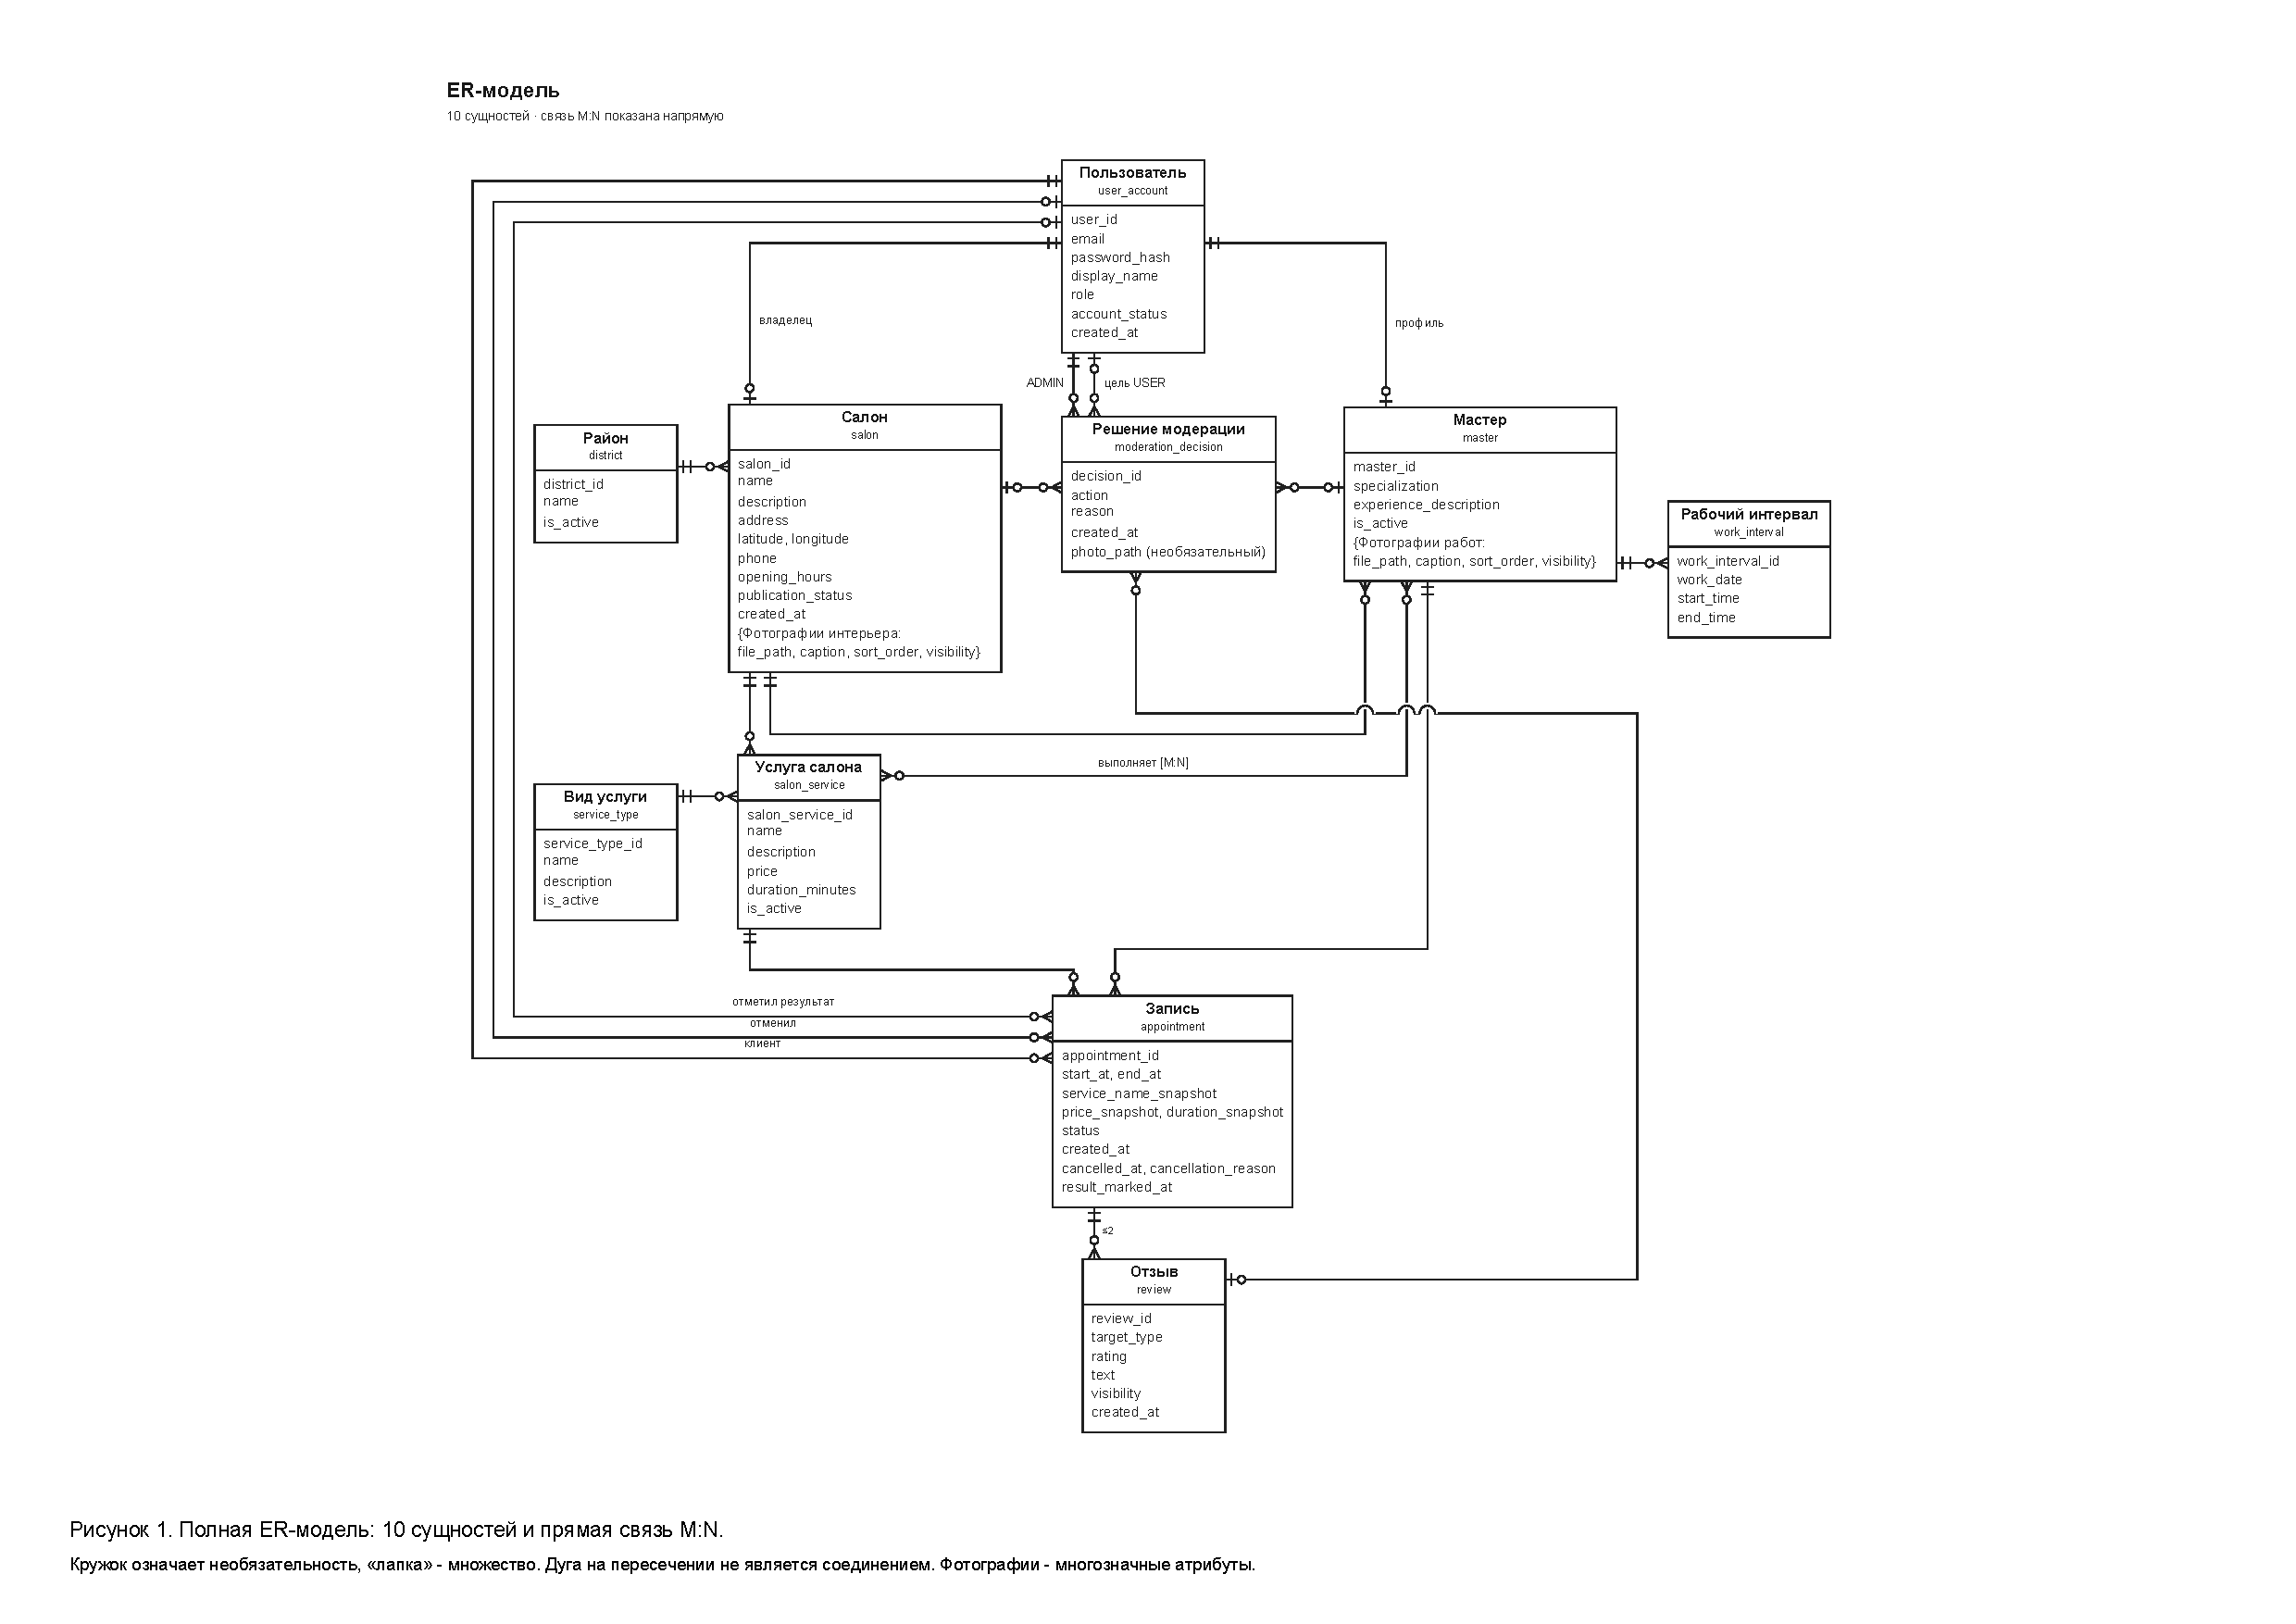
\includepdf[pages=1,fitpaper=true,pagecommand={\thispagestyle{empty}}]{figures/er_model_a3.pdf}
\section{Даталогическая модель и нормализация}
Полная схема на рисунке~2 содержит \textbf{14 таблиц}: десять основных отношений, таблицу связи M:N, две таблицы элементов фотоатрибутов и техническую таблицу приглашений.


\begin{longtable}{L{4.1cm}L{12.0cm}}
\toprule Преобразование & Результат и ключ\\\midrule\endhead
Бизнес-сущности & По одной таблице с идентификатором; исключение для многозначных атрибутов указано ниже.\\
Связь M:N & \texttt{master\_\allowbreak{}service}: PK (master\_id, salon\_service\_id), активность пары.\\
Фотографии & \texttt{salon\_\allowbreak{}photo}, \texttt{master\_\allowbreak{}photo}: составные PK (родитель, file\_path).\\
Одноразовое приглашение & \texttt{master\_\allowbreak{}invitation}: invitation\_id; уникальный хеш, срок, использование и отзыв токена.\\
\bottomrule\end{longtable}


Запись ссылается составным FK на разрешённую пару «мастер--услуга». Триггер дополнительно проверяет принадлежность обоих объектов одному салону. Отзыв имеет FK на запись и уникальную пару (appointment\_id, target\_type): не более одного отзыва о салоне и одного о мастере. Имя мастера хранится в пользователе и не дублируется в профиле.

Для модерации используются четыре целевых FK с XOR. Два дополнительных составных FK (target\_salon\_id, photo\_path) и (target\_master\_id, photo\_path) проверяют существование конкретного фотоэлемента. Все внешние ключи используют ON DELETE RESTRICT: исторически значимые объекты архивируются.

Разделение фотоэлементов устраняет повторяющиеся группы и обеспечивает 1НФ. Атрибуты основных отношений зависят от их ключей; связи и сведения о пользователе не дублируются, что соответствует 3НФ. Снимки названия, цены и длительности относятся к факту подтверждения записи и сохраняют историю. Окончание и диапазон времени --- контролируемые generated-столбцы. Рейтинги и свободные времена вычисляются запросами.

На рисунке~2 ключи вынесены в отдельную левую колонку; типы справа выделены полужирным. PK --- первичный ключ, FK --- внешний, UQ --- уникальность, NN --- NOT NULL, G --- вычисляемый столбец. Повтор F13 у двух полей означает один составной FK, а не две независимые ссылки.
\clearpage
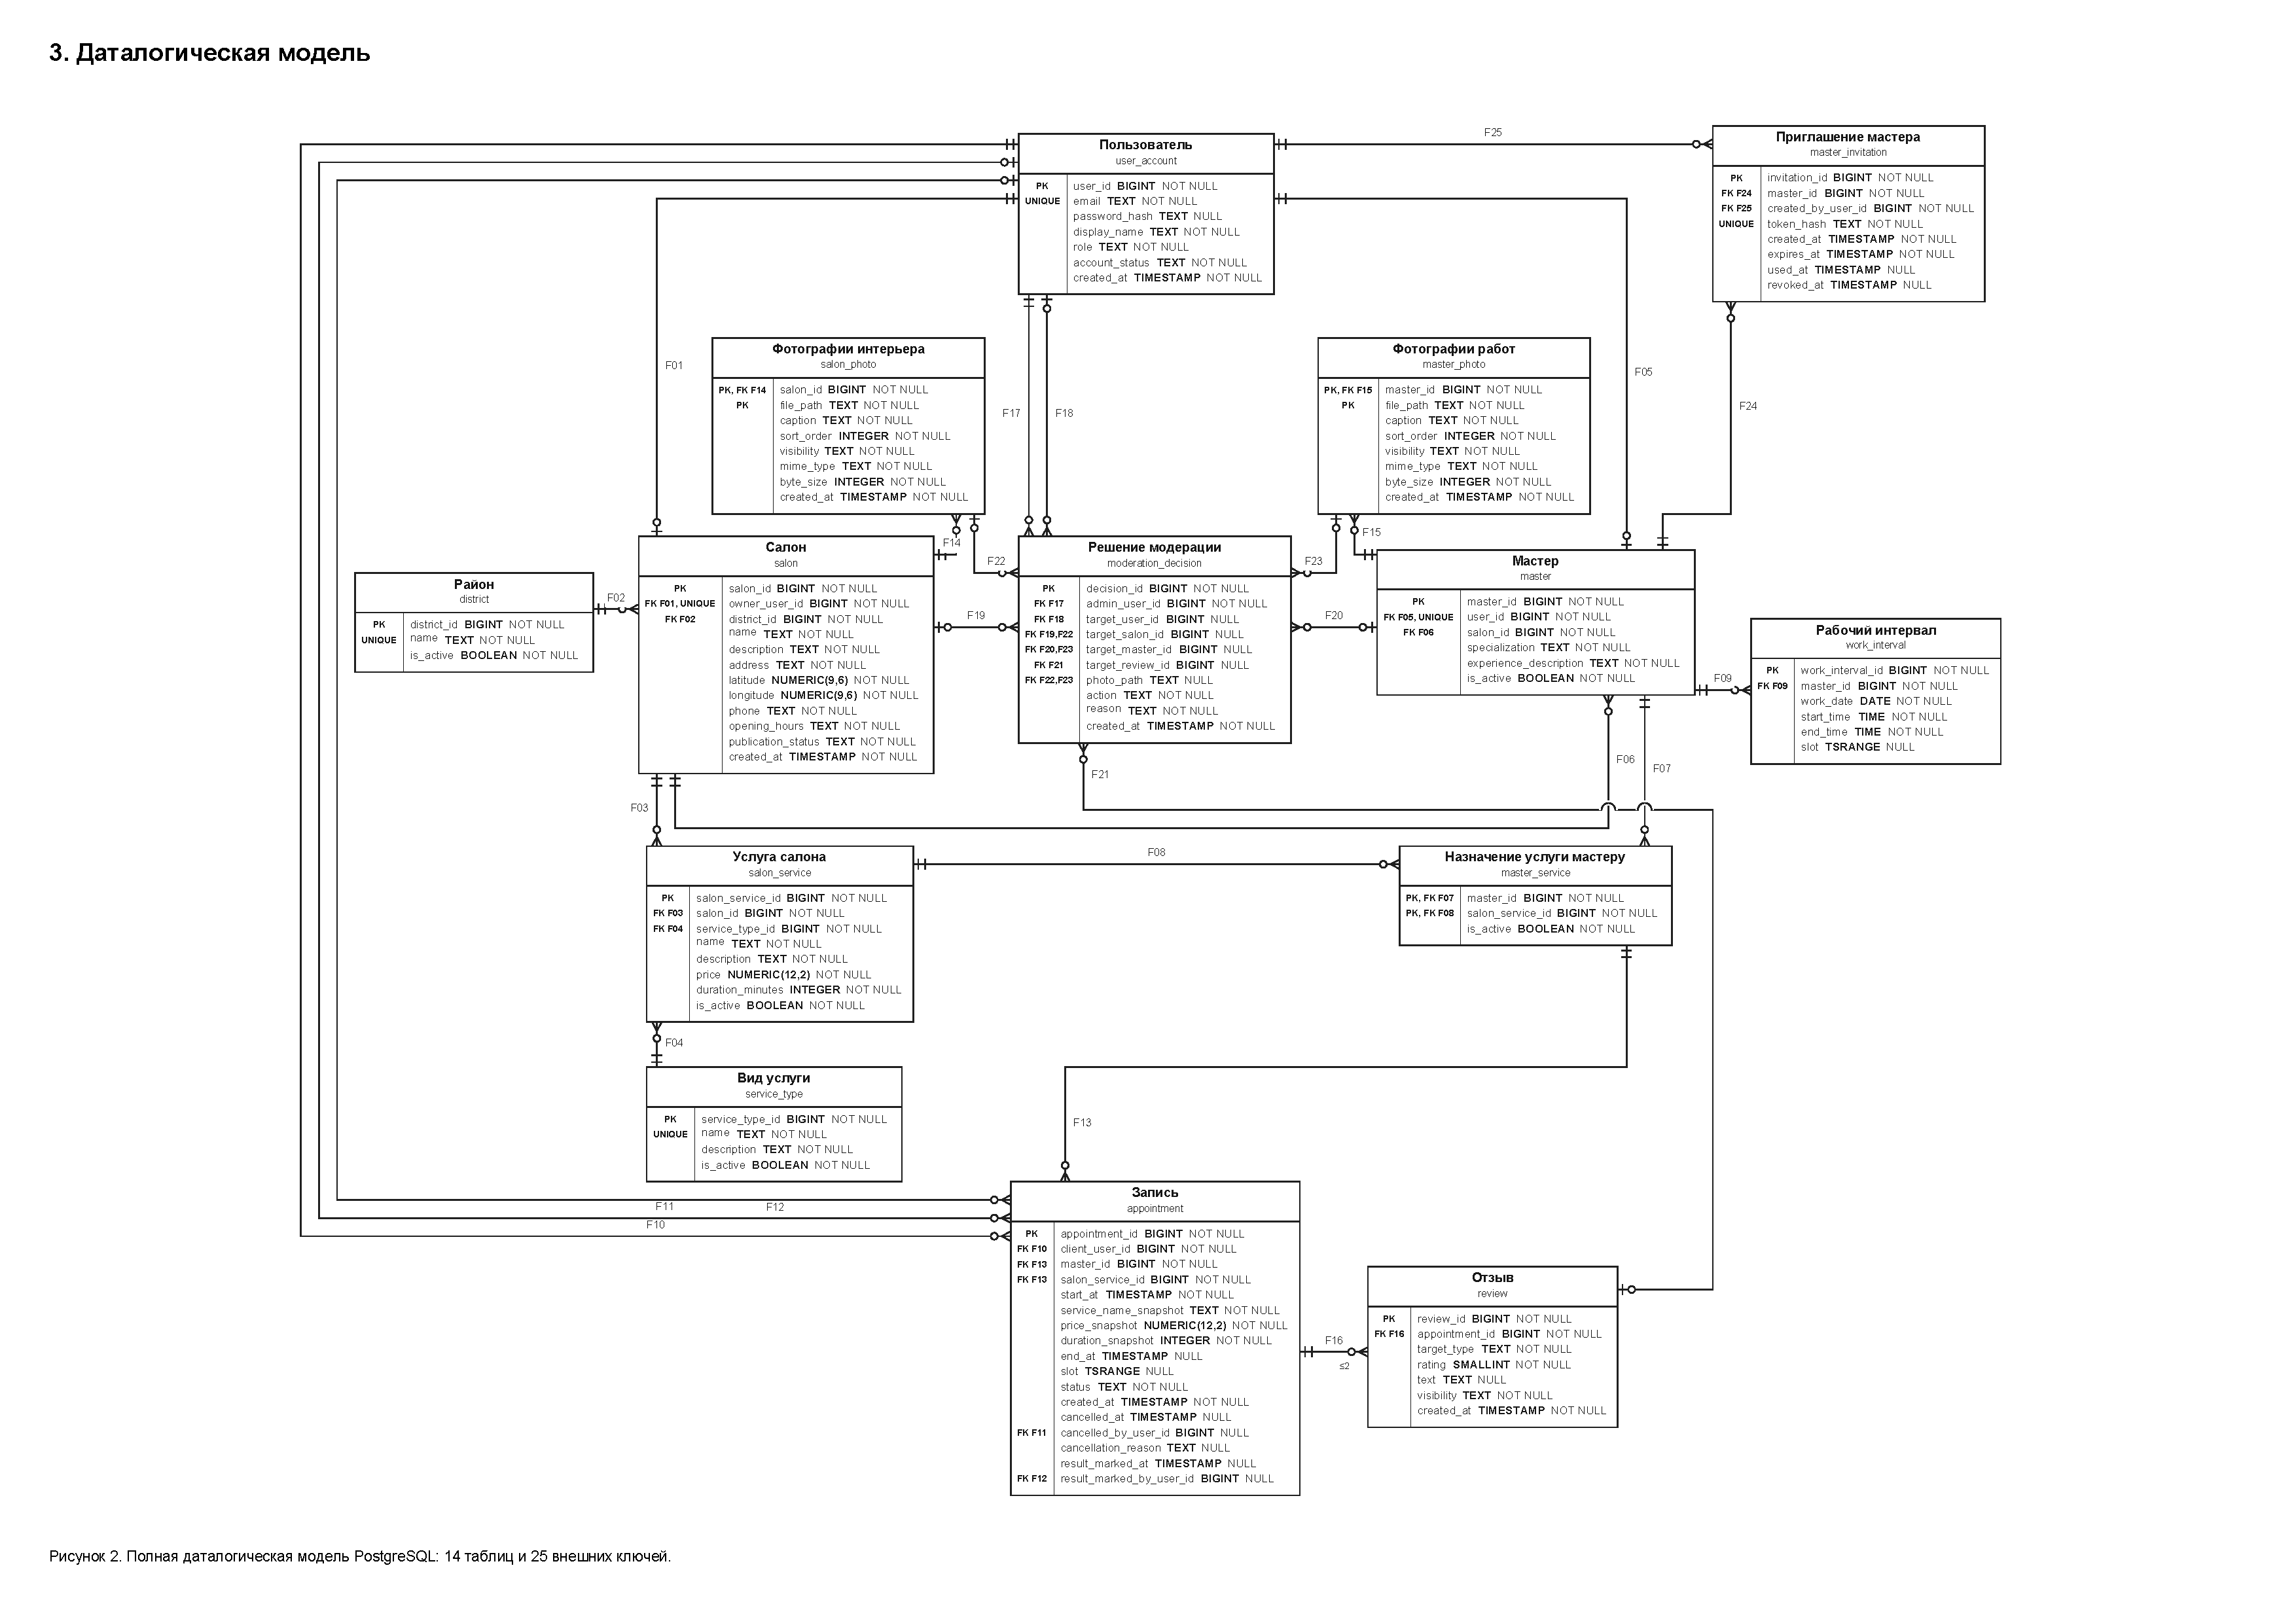
\includepdf[pages=1,fitpaper=true,pagecommand={\thispagestyle{empty}}]{figures/logical_model_a2.pdf}
\section{Целостность и доступ}


\begin{longtable}{L{4.1cm}L{12.0cm}}
\toprule Инвариант & Реализация\\\midrule\endhead
Идентичность и принадлежность & PK, FK, UQ; неизменность роли и владельческих связей; проверка ролей и одного салона триггерами.\\
Нет пересечения времени & GiST EXCLUDE по мастеру и диапазону для рабочих интервалов и неотменённых записей. Полуоткрытые интервалы допускают соседние посещения.\\
Запись допустима & Триггер проверяет публикацию, активность, разрешённую пару, горизонт, шаг начала и вхождение всей услуги в один рабочий интервал.\\
История и статусы & Снимки неизменны; отмена до начала, результат после окончания. Сокращение графика и деактивация не нарушают ещё не завершённые подтверждённые записи.\\
Отзывы и модерация & Только COMPLETED, рейтинг 1--5, UQ по типу цели; неизменяемый текст и аудит. CHECK XOR и составные FK для фото.\\
Фото и приглашения & До 20 неархивных фото; JPEG/PNG до 5 МБ; скрытые фото учитываются в квоте. Уникальный одноразовый токен, срок и взаимное исключение использования и отзыва.\\
\bottomrule\end{longtable}

Основные фрагменты DDL:

\begin{lstlisting}[style=sql]
CREATE TABLE beauty.master_service (
  master_id bigint NOT NULL
    REFERENCES beauty.master ON DELETE RESTRICT,
  salon_service_id bigint NOT NULL
    REFERENCES beauty.salon_service ON DELETE RESTRICT,
  is_active boolean NOT NULL DEFAULT true,
  PRIMARY KEY (master_id, salon_service_id)
);

-- Constraint inside beauty.appointment:
CONSTRAINT ex_appointment_overlap
  EXCLUDE USING gist (master_id WITH =, slot WITH &&)
  WHERE (status <> 'CANCELLED')
\end{lstlisting}


Триггеры защищают условия, зависящие от других строк и времени. Например, контроль права на отзыв включает следующую проверку:


\begin{lstlisting}[style=sql]
IF NOT EXISTS (
  SELECT FROM beauty.appointment
  WHERE appointment_id = NEW.appointment_id
    AND status = 'COMPLETED'
) THEN
  RAISE EXCEPTION 'Review requires a completed visit'
    USING ERRCODE = '23514';
END IF;
\end{lstlisting}


Все бизнес-записи получают единый транзакционный advisory lock до чтения изменяемых условий и блокировки строк. Допускается READ COMMITTED; иной уровень явно отклоняется. Это устраняет проверяемые гонки между записью, графиком, каталогом и токенами, но последовательно выполняет изменения всей платформы. Производительность при 20 параллельных клиентах не подтверждена; для масштабирования требуется более мелкая схема блокировок.

Backend получает только EXECUTE на API; актор берётся из аутентифицированной сессии. Проверку файлов выполняет файловый сервис.

\section{Критические функции и процедуры}
Реализованы 22 бизнес-операции. Пишущие операции используют PL/pgSQL; выбор свободного времени выражен SQL-запросом. Два view рассчитывают независимые рейтинги салона и мастера только по опубликованным отзывам.


\begin{longtable}{L{2.8cm}L{13.3cm}}
\toprule Прецеденты & API и назначение\\\midrule\endhead
П1 & \texttt{register\_\allowbreak{}user}, \texttt{authenticate}: регистрация и пароль; \texttt{accept\_\allowbreak{}invitation}: активация мастера.\\
П2--П4, П12 & \texttt{search\_\allowbreak{}salons}, \texttt{available\_\allowbreak{}slots}, \texttt{book\_\allowbreak{}appointment}: фильтры, допустимые начала и подтверждение условий.\\
П5, П9, П10 & \texttt{appointment\_\allowbreak{}journal}, \texttt{cancel\_\allowbreak{}appointment}, \texttt{mark\_\allowbreak{}visit}: личная история, отмена и результат посещения.\\
П6, П7, П11 & \texttt{add\_\allowbreak{}review}, \texttt{moderate}, \texttt{create\_\allowbreak{}salon}, \texttt{resubmit\_\allowbreak{}salon}: отзывы, решения и публикация.\\
П8, П9 & \texttt{invite\_\allowbreak{}master}, \texttt{reissue\_\allowbreak{}invitation}, \texttt{set\_\allowbreak{}master\_\allowbreak{}service}, \texttt{save\_\allowbreak{}work\_\allowbreak{}interval}, \texttt{delete\_\allowbreak{}work\_\allowbreak{}interval}, \texttt{save\_\allowbreak{}service}, \texttt{save\_\allowbreak{}master\_\allowbreak{}profile}, \texttt{put\_\allowbreak{}photo}, \texttt{archive\_\allowbreak{}photo}: управление своим салоном и профилем.\\
\bottomrule\end{longtable}


При подтверждении записи сервер повторно проверяет цену и длительность: изменение каталога требует нового подтверждения клиента. После INSERT триггер проверяет доступность и сохраняет актуальные снимки. Полный пример критической функции:


\begin{lstlisting}[style=sql]
CREATE FUNCTION beauty.book_appointment(
  p_client bigint, p_master bigint, p_service bigint,
  p_start timestamp, p_expected_price numeric,
  p_expected_duration integer
) RETURNS bigint
LANGUAGE plpgsql SECURITY DEFINER
SET search_path = pg_catalog, beauty, pg_temp AS $$
DECLARE s beauty.salon_service; id bigint;
BEGIN
  PERFORM beauty.lock_writes();
  PERFORM beauty.require_actor(p_client, ARRAY['CLIENT']);
  SELECT * INTO s FROM beauty.salon_service
    WHERE salon_service_id = p_service;
  IF NOT FOUND THEN RAISE EXCEPTION 'Service does not exist'
    USING ERRCODE = '23503'; END IF;
  IF s.price IS DISTINCT FROM p_expected_price OR
     s.duration_minutes IS DISTINCT FROM p_expected_duration THEN
    RAISE EXCEPTION 'Service terms changed; confirm again'
      USING ERRCODE = '22023'; END IF;
  INSERT INTO beauty.appointment (
    client_user_id, master_id, salon_service_id, start_at,
    service_name_snapshot, price_snapshot, duration_snapshot
  ) VALUES (
    p_client, p_master, p_service, p_start,
    s.name, s.price, s.duration_minutes
  ) RETURNING appointment_id INTO id;
  RETURN id;
END $$;
\end{lstlisting}


Процедура mark\_visit принимает только COMPLETED или NO\_SHOW; триггер проверяет полномочия конкретного мастера/владельца и наступление планового окончания. cancel\_appointment идемпотентна, сохраняет автора и причину и освобождает слот. add\_review проверяет принадлежность завершённого посещения клиенту. Приглашение хранит хеш; повторная выдача отзывает прежний токен, активация использует его ровно один раз.

\section{Индексы по прецедентам}
В схеме 43 индекса: 23 обеспечивают PK/UQ/EXCLUDE, 19 созданы для запросов и один частичный уникальный индекс защищает открытые приглашения. Индексы ограничений не дублируются.


\begin{longtable}{L{6.4cm}L{2.0cm}L{7.3cm}}
\toprule Индекс & Прецедент & Польза\\\midrule\endhead
\texttt{idx\_\allowbreak{}salon\_\allowbreak{}public\_\allowbreak{}district} & П2 & Район и идентификатор в опубликованном каталоге.\\
\texttt{idx\_\allowbreak{}salon\_\allowbreak{}public\_\allowbreak{}coordinates} & П2 & Отбор прямоугольника карты; радиус вычисляется для кандидатов.\\
\texttt{idx\_\allowbreak{}service\_\allowbreak{}salon\_\allowbreak{}type\_\allowbreak{}price} & П2, П3 & Тип и цена услуги внутри выбранного салона.\\
\texttt{idx\_\allowbreak{}service\_\allowbreak{}type\_\allowbreak{}price} & П2 & Поиск салонов по типу и диапазону цены одной услуги.\\
\texttt{idx\_\allowbreak{}master\_\allowbreak{}salon} & П3, П8 & Активные мастера салона.\\
\texttt{idx\_\allowbreak{}assignment\_\allowbreak{}service} & П3, П4 & Мастера услуги; обратный порядок к PK связи M:N.\\
\texttt{idx\_\allowbreak{}work\_\allowbreak{}master\_\allowbreak{}date} & П4, П9, П12 & График мастера в нужную дату; INCLUDE окончания.\\
\texttt{idx\_\allowbreak{}appointment\_\allowbreak{}client\_\allowbreak{}time} & П5 & Последние записи клиента без полной сортировки.\\
\texttt{idx\_\allowbreak{}appointment\_\allowbreak{}master\_\allowbreak{}time} & П9, П10 & Журнал мастера за дату и история посещений.\\
\texttt{idx\_\allowbreak{}appointment\_\allowbreak{}service\_\allowbreak{}future} & П8 & Проверка защиты услуги с будущими подтверждёнными записями.\\
\texttt{idx\_\allowbreak{}appointment\_\allowbreak{}busy} & П4, П12 & GiST-поиск пересекающихся подтверждённых интервалов.\\
\texttt{idx\_\allowbreak{}review\_\allowbreak{}published\_\allowbreak{}target} & П3, П6, П11 & Опубликованные оценки нужного типа цели.\\
\texttt{idx\_\allowbreak{}salon\_\allowbreak{}photo\_\allowbreak{}visible}\par \texttt{idx\_\allowbreak{}master\_\allowbreak{}photo\_\allowbreak{}visible} & П3 & Видимые фото родителя в порядке показа.\\
\texttt{idx\_\allowbreak{}moderation\_\allowbreak{}user}\par \texttt{idx\_\allowbreak{}moderation\_\allowbreak{}salon}\par \texttt{idx\_\allowbreak{}moderation\_\allowbreak{}master}\par \texttt{idx\_\allowbreak{}moderation\_\allowbreak{}review} & П7, П11 & История решений по конкретному объекту; частичные индексы без NULL.\\
\texttt{idx\_\allowbreak{}invitation\_\allowbreak{}master\_\allowbreak{}history} & П1, П8 & История и повторная выдача приглашений мастера.\\
\texttt{uq\_\allowbreak{}invitation\_\allowbreak{}open} & П1 & Не более одного неиспользованного, неотозванного токена.\\
\bottomrule\end{longtable}

Примеры индексов для истории клиента и поиска занятых слотов:

\begin{lstlisting}[style=sql]
CREATE INDEX idx_appointment_client_time
  ON beauty.appointment (client_user_id, start_at DESC)
  INCLUDE (status, master_id, salon_service_id);

CREATE INDEX idx_appointment_busy
  ON beauty.appointment USING gist (master_id, slot)
  WHERE status = 'CONFIRMED';
\end{lstlisting}


B-tree обслуживает равенства, диапазоны и сортировку; GiST --- пересечение диапазонов. Частичные индексы исключают неактуальные строки. Индекс координат ускоряет предварительный отбор, а не сам расчёт географического расстояния. В малых справочниках последовательное сканирование может быть выгоднее индекса.

\section{Скрипты и воспроизведение}
Нужны PostgreSQL, psql, права владельца схемы и расширения btree\_gist, pgcrypto. Проверенная версия --- PostgreSQL 17.4. При работе в выданной преподавателем пустой базе шаг CREATE DATABASE пропускается.


\begin{longtable}{L{8.1cm}L{8.0cm}}
\toprule Файлы & Назначение\\\midrule\endhead
\texttt{sql/00\_\allowbreak{}create\_\allowbreak{}database.\allowbreak{}sql}, \texttt{sql/99\_\allowbreak{}drop\_\allowbreak{}database.\allowbreak{}sql} & Создание явно указанной UTF-8 базы и удаление без FORCE.\\
\texttt{sql/01\_\allowbreak{}tables.\allowbreak{}sql}, \texttt{sql/02\_\allowbreak{}seed.\allowbreak{}sql} & Таблицы, декларативные ограничения и синтетические данные.\\
\texttt{sql/03\_\allowbreak{}integrity.\allowbreak{}sql}, \texttt{sql/04\_\allowbreak{}routines.\allowbreak{}sql} & Триггеры, помощники, бизнес-функции, процедуры и view.\\
\texttt{sql/05\_\allowbreak{}indexes.\allowbreak{}sql}, \texttt{sql/06\_\allowbreak{}grant\_\allowbreak{}backend.\allowbreak{}sql} & Индексы запросов и EXECUTE для существующей серверной роли.\\
\texttt{sql/install.\allowbreak{}sql} & Атомарная установка, необязательные демоданные и ANALYZE.\\
\texttt{scripts/CreateDatabase.\allowbreak{}ps1}, \texttt{scripts/DropDatabase.\allowbreak{}ps1}, \texttt{scripts/TestDatabase.\allowbreak{}ps1} & Локальные команды создания, удаления и изолированной проверки.\\
\bottomrule\end{longtable}

Запуск из каталога второго этапа:

\begin{lstlisting}[style=commands]
psql -h HOST -U USER -d postgres \
  -v db_name=beauty_course -f sql/00_create_database.sql
psql -h HOST -U USER -d beauty_course \
  -v with_demo_data=true -f sql/install.sql
psql -h HOST -U OWNER -d beauty_course \
  -v backend_role=SERVER_ROLE -f sql/06_grant_backend.sql
psql -h HOST -U USER -d postgres \
  -v db_name=beauty_course -f sql/99_drop_database.sql
\end{lstlisting}
Исторические демоданные загружаются после DDL, до установки бизнес-триггеров, в одной транзакции install. Декларативные ограничения действуют при загрузке; дополнительные проверки подтверждают согласованность истории. Этот путь предназначен для новой демонстрационной базы. Без флага демоданных создаётся пустая рабочая схема. Удаление не завершает чужие сеансы.

\section{Результаты проверки}


Выполнено \textbf{79 из 79 проверок}; все завершились успешно. Создано 14 таблиц, 32 пользовательских триггера, 43 индекса. Проверены установка с демоданными и без них, создание и удаление отдельной базы, допустимые и запрещённые сценарии и права backend.

\begin{longtable}{L{4.2cm}L{11.9cm}}
\toprule Данные / проверка & Результат\\\midrule\endhead
Нагрузка тестовых данных & 100 салонов, 501 профиль мастера, 600 услуг; 80000 рабочих интервалов, 50005 записей, 12000 отзывов.\\
Время и каталог & Отклонены пересечение, перерыв, прошедшая дата, неверный шаг, чужая услуга и изменение занятых условий; соседние записи разрешены.\\
Права и история & Отклонены чужая отмена, ранний результат, изменение конечного статуса, удаление истории, повтор отзыва, прямой доступ к таблицам.\\
Модерация и приглашения & Проверены XOR, ссылки на фото, квота, скрытие и рейтинги, сроки, отзыв и одноразовое использование токена.\\
Четыре конкурентных сценария & Повтор одной записи; запись против сокращения графика; одинаковый отзыв; двойная активация приглашения.\\
\bottomrule\end{longtable}


В конкурентных проверках использованы пары реальных сеансов: первая транзакция удерживалась две секунды, вторая ожидала блокировку более секунды. Вторая запись в тот же слот отклонялась с 23P01, сокращение занятого графика --- с 23514, повтор отзыва --- с 23505, повтор токена --- с 22023. Проверка нагрузки всей платформы не проводилась.

EXPLAIN (ANALYZE, BUFFERS, FORMAT JSON) выполнен без отключения последовательного сканирования:


\begin{longtable}{L{4.0cm}L{9.8cm}L{1.8cm}}
\toprule Запрос & Выбранные индексы & мс\\\midrule\endhead
История клиента & \texttt{idx\_\allowbreak{}appointment\_\allowbreak{}client\_\allowbreak{}time} & 0.159\\
Журнал мастера & \texttt{idx\_\allowbreak{}appointment\_\allowbreak{}master\_\allowbreak{}time} & 0.883\\
График на дату & \texttt{idx\_\allowbreak{}work\_\allowbreak{}master\_\allowbreak{}date} & 0.51\\
Пересечение слота & \texttt{idx\_\allowbreak{}appointment\_\allowbreak{}busy}\par \texttt{idx\_\allowbreak{}appointment\_\allowbreak{}master\_\allowbreak{}time} & 1.777\\
Тип услуги и цена & \texttt{idx\_\allowbreak{}service\_\allowbreak{}type\_\allowbreak{}price} & 0.141\\
\bottomrule\end{longtable}


Планы подтверждают использование индексов в пяти характерных запросах. Время относится к локальным SQL-вызовам и не включает сеть, HTTP или параллельную нагрузку. Геометрическая проверка двух полных схем подтвердила отсутствие повторных сущностей, перекрытий и проходов через рамки; три и два пересечения соответственно обозначены дугами.

\section{Заключение}
Построены ER-модель из десяти сущностей с M:N и даталогическая модель из четырнадцати отношений. Реализованы PostgreSQL DDL, триггеры, бизнес-операции PL/pgSQL, индексы и скрипты жизненного цикла. Все 79 проверок пройдены; полезность индексов подтверждена планами запросов. Материалы готовы к обсуждению с преподавателем; фактическое согласование ER-модели остаётся обязательным внешним шагом.
\end{document}
